\chapter{细胞代谢}\label{ch:g10:cell-metabolism}

取一只气球套在烧瓶瓶口上，烧瓶中盛有加了一勺面包酵母的温热糖水。
不到一小时，液体变得浑浊并冒泡，气球鼓了起来，
烧瓶里还隐约飘出面包和啤酒的气味。
酵母\omterm{def:g10:cells-common-unit:cell}{细胞}正在分解\omterm{def:g10:chemistry-of-life:families}{糖类}，并将其转变为别的物质，
释放出的气体与你呼出的二氧化碳相同。
阳光下的叶片则正好相反：吸收二氧化碳，释放氧气。
两者都是在\omterm{def:g10:cells-common-unit:cell}{细胞}内进行的化学过程，温度与体温相当，
不需要明火，也不需要酸——
本章讨论的正是这类化学过程。

\section{代谢：细胞中的化学}

\begin{definition}[代谢]\label{def:g10:cell-metabolism:metabolism}
\omterm{def:g10:cells-common-unit:cell}{细胞}的\emph{代谢}\index{代谢}是指\omterm{def:g10:cells-common-unit:cell}{细胞}内发生的全部
化学反应的总和，其中既有分解分子以释放能量的反应，
也有由较简单的分子合成\omterm{def:g10:cells-common-unit:cell}{细胞}自身所需分子的反应。
代谢中的每一个反应都由
\emph{酶}\index{酶}催化，酶是一种能加快某一特定反应速率的\omterm{def:g10:chemistry-of-life:families}{蛋白质}，
自身在反应中不被消耗。
\end{definition}

\begin{proposition}[酶使细胞化学成为可能]\label{prop:g10:cell-metabolism:enzymes}
葡萄糖置于 \qty{37}{\celsius} 的空气中不会燃烧；在\omterm{def:g10:cells-common-unit:cell}{细胞}内，
它却会在几分钟内被彻底氧化。两者的差别在于酶：每一种酶
都与特定的分子（即其\emph{底物}）结合，将其转变为
产物，随后释放并重新开始，每秒可重复数千次。
因此，\omterm{def:g10:cells-common-unit:cell}{细胞}的\omterm{def:g10:cell-metabolism:metabolism}{代谢}由其所具有的一整套酶决定，
而这套酶又由\omterm{def:g10:universal-dna:gene}{基因}决定。
\end{proposition}
\admitted

\begin{example}[一种酶的作用]\label{ex:g10:cell-metabolism:catalase}
将过氧化氢滴在一小块生肝或生土豆上，会剧烈起泡，
同时释放出氧气。几乎每个\omterm{def:g10:cells-common-unit:cell}{细胞}中都含有过氧化氢酶，
它能将有毒的过氧化氢分解为水和氧气，
每个酶分子每秒可分解数百万个过氧化氢分子。先煮沸肝脏，则不会发生任何反应：
酶是\omterm{def:g10:chemistry-of-life:families}{蛋白质}，已被热量破坏。
滴在石块上的过氧化氢不起泡，说明
该反应不会自发进行。
\end{example}

\begin{omfigure}
\begin{tikzpicture}[>=Stealth, font=\small]
  \node[draw, rounded corners, fill=omDef!15, minimum width=1.6cm, minimum height=1.1cm] (e1) at (0,0) {酶};
  \node[draw, fill=omProp!30, minimum width=0.9cm, minimum height=0.5cm] (s) at (0,1.3) {底物};
  \draw[->] (s) -- (e1);
  \node[draw, rounded corners, fill=omDef!15, minimum width=1.6cm, minimum height=1.1cm] (e2) at (4,0) {酶};
  \node[draw, fill=omProp!30, minimum width=0.9cm, minimum height=0.5cm, anchor=south] (s2) at (4,0.55) {底物};
  \draw[->] (e1.east) -- node[above] {结合} (e2.west);
  \node[draw, rounded corners, fill=omDef!15, minimum width=1.6cm, minimum height=1.1cm] (e3) at (8,0) {酶};
  \node[draw, fill=omMeth!30, minimum width=0.5cm, minimum height=0.5cm] (p1) at (7.5,1.5) {产物};
  \node[draw, fill=omMeth!30, minimum width=0.5cm, minimum height=0.5cm] (p2) at (9.1,1.5) {产物};
  \draw[->] (e2.east) -- node[above] {转化} (e3.west);
  \draw[->] (e3.north) -- (p1.south);
  \draw[->] (e3.north) -- (p2.south);
  \draw[->, dashed] (e3.south) to[bend left=25] node[below] {释放，自身不变，重新开始} (e1.south);
\end{tikzpicture}

{\small 酶与底物结合，将其转化并释放出
产物，酶本身保持不变。一个酶分子每秒可
重复此循环数千次。}
\end{omfigure}

\section{细胞获取营养的两种方式}

\begin{definition}[自养与异养]\label{def:g10:cell-metabolism:autotrophy}
若\omterm{def:g10:cells-common-unit:cell}{细胞}仅由\omterm{def:g10:chemistry-of-life:mineral-organic}{无机物}合成自身的有机分子，则称其为\emph{自养}\index{自养}的，
即以二氧化碳、水和\omterm{def:g10:chemistry-of-life:mineral-organic}{无机盐}为原料，并利用外界能量。
带\omterm{def:g10:cells-common-unit:organelle}{叶绿体}的植物\omterm{def:g10:cells-common-unit:cell}{细胞}、藻类和部分细菌都是自养\omterm{def:g10:cells-common-unit:cell}{细胞}，
其能量来自光，
这一过程即为\emph{光合作用}\index{光合作用}。
若\omterm{def:g10:cells-common-unit:cell}{细胞}必须摄取其他生物制造的有机分子，则称其为\emph{异养}\index{异养}的，
这些有机分子既用作建造材料，也用作能量来源。动物\omterm{def:g10:cells-common-unit:cell}{细胞}、真菌、
大多数细菌，以及植物中非绿色的\omterm{def:g10:cells-common-unit:cell}{细胞}（如根\omterm{def:g10:cells-common-unit:cell}{细胞}），
均为异养\omterm{def:g10:cells-common-unit:cell}{细胞}。
\end{definition}

\begin{proposition}[光合作用]\label{prop:g10:cell-metabolism:photosynthesis}
在光照下，含\omterm{def:g10:cells-common-unit:organelle}{叶绿体}的\omterm{def:g10:cells-common-unit:cell}{细胞}吸收二氧化碳和
水，释放氧气，并合成葡萄糖，葡萄糖随后转化为
淀粉、纤维素、\omterm{def:g10:chemistry-of-life:families}{脂质}，并在无机氮参与下合成\omterm{def:g10:chemistry-of-life:families}{氨基酸}。概括来说，
\omterm{def:g10:cell-metabolism:autotrophy}{光合作用}的总反应式为：
\[
6\,\mathrm{CO_2} + 6\,\mathrm{H_2O} \xrightarrow{\ \text{光、叶绿素}\ }
\mathrm{C_6H_{12}O_6} + 6\,\mathrm{O_2}.
\]
光能储存在葡萄糖的化学键之中。
\end{proposition}
\begin{proof}[证据]
将绿藻\emph{Chlorella}的悬浮液置于一个密闭容器中，
容器装有氧气探头，实验结果显示，
开灯时溶解氧持续上升，关灯时下降；若除去水中的
二氧化碳，溶解氧的上升便会停止。将叶片在黑暗中
放置两天后，遇碘不再呈蓝黑色；另取一片叶子，一半用锡箔遮盖，
只有暴露的一半显色，说明淀粉生成于有光照射之处。
向植物供给放射性二氧化碳，
几分钟内即出现在植物的\omterm{def:g10:chemistry-of-life:families}{糖类}中。
\end{proof}

\begin{omfigure}
\begin{tikzpicture}
\begin{axis}[
  width=0.88\linewidth, height=5.4cm,
  axis x line=bottom, axis y line=left,
  xmin=0, xmax=22, ymin=5, ymax=13,
  xlabel={时间（min）}, ylabel={溶解氧 $\mathrm{O_2}$（mg/L）},
  xlabel style={font=\small, at={(axis description cs:0.5,-0.12)}, anchor=north},
  ylabel style={font=\small},
  tick label style={font=\small}, xtick={0,5,10,15,20},
  clip=false,
]
\addplot[thick, omMeth] coordinates {(0,8.0) (5,8.0) (10,10.5) (15,10.0) (20,12.5)};
\draw[dashed, gray] (axis cs:5,5) -- (axis cs:5,13);
\draw[dashed, gray] (axis cs:10,5) -- (axis cs:10,13);
\draw[dashed, gray] (axis cs:15,5) -- (axis cs:15,13);
  \node[font=\small, anchor=south] at (axis cs:2.5,12.5) {黑暗};
  \node[font=\small, anchor=south] at (axis cs:7.5,12.5) {光照};
  \node[font=\small, anchor=south] at (axis cs:12.5,12.5) {黑暗};
  \node[font=\small, anchor=south] at (axis cs:17.5,12.5) {光照};
\end{axis}
\end{tikzpicture}

{\small 密闭的 \emph{Chlorella} 悬浮液中的溶解氧。
光照下，藻类释放氧气的速度快于其消耗速度；
黑暗中仅剩呼吸作用，氧气含量下降。每条斜线
即为一种速率，以毫克每升每分钟读出。}
\end{omfigure}

\begin{example}[Euglena 兼具两种营养方式]\label{ex:g10:cell-metabolism:euglena}
单\omterm{def:g10:cells-common-unit:cell}{细胞}的 \emph{Euglena} 具有\omterm{def:g10:cells-common-unit:organelle}{叶绿体}，借一根
鞭毛游动。光照下，于\omterm{def:g10:chemistry-of-life:mineral-organic}{无机盐}水中，它能生长，属\omterm{def:g10:cell-metabolism:autotrophy}{自养}型。
黑暗中，只有在水中加入有机分子，它才能存活，
它吸收这些分子，属\omterm{def:g10:cell-metabolism:autotrophy}{异养}型。长期处于黑暗中，它会失去
\omterm{def:g10:cells-common-unit:organelle}{叶绿体}；移回光照下，经过几天它便
重新长出\omterm{def:g10:cells-common-unit:organelle}{叶绿体}。它的\omterm{def:g10:cell-metabolism:metabolism}{代谢}取决于允许两种方式的\omterm{def:g10:universal-dna:gene}{基因}，
也取决于环境，环境会选择其中一种。
\end{example}

\section{从有机分子中获取能量}

\begin{proposition}[细胞呼吸]\label{prop:g10:cell-metabolism:respiration}
所有\omterm{def:g10:cells-common-unit:cell}{细胞}，无论\omterm{def:g10:cell-metabolism:autotrophy}{自养}还是\omterm{def:g10:cell-metabolism:autotrophy}{异养}，都通过分解
有机分子获取可用能量。有氧存在时，分解
彻底——此即\emph{细胞呼吸}\index{细胞呼吸}
，发生于\omterm{def:g10:cells-common-unit:organelle}{线粒体}中：
\[
\mathrm{C_6H_{12}O_6} + 6\,\mathrm{O_2} \longrightarrow
6\,\mathrm{CO_2} + 6\,\mathrm{H_2O} + \text{能量},
\]
每摩尔葡萄糖（\qty{180}{g}）约释放 \qty{2870}{kJ} 能量，其中
约 40\% 储存于一种小分子中，
\emph{ATP}\index{ATP}，\omterm{def:g10:cells-common-unit:cell}{细胞}中每个耗能过程——
运动、运输、合成——都依赖于它；其余的能量
以热量的形式释放。
\end{proposition}
\begin{proof}[证据]
装有氧探头的密闭容器中，酵母在
饥饿时不耗氧；加入葡萄糖后，溶解氧以稳定速率下降，
同时出现二氧化碳，直至氧气耗尽。发芽的
种子置于真空保温瓶中，一天之内使瓶子升温数摄氏度
——即呼吸作用产生的热量——而煮沸过的种子则没有。肌肉\omterm{def:g10:cells-common-unit:cell}{细胞}
在电子显微镜下，可见其中挤满\omterm{def:g10:cells-common-unit:organelle}{线粒体}，而
一种\omterm{def:g10:cells-common-unit:organelle}{线粒体}毒物会使肌肉停止收缩。
\end{proof}

\begin{omfigure}
\begin{tikzpicture}
\begin{axis}[
  width=0.88\linewidth, height=5.4cm,
  axis x line=bottom, axis y line=left,
  xmin=0, xmax=12, ymin=0, ymax=10,
  xlabel={时间 (min)}, ylabel={溶解 $\mathrm{O_2}$ (mg/L)},
  xlabel style={font=\small, at={(axis description cs:0.5,-0.12)}, anchor=north},
  ylabel style={font=\small},
  tick label style={font=\small}, xtick={0,2,4,6,8,10,12},
  clip=false,
]
\addplot[thick, omThm] coordinates {(0,8.0) (3,7.9) (10,0.9) (12,0.6)};
\draw[->, thick] (axis cs:3,9.6) -- (axis cs:3,8.3);
\node[font=\small, anchor=south] at (axis cs:3,9.7) {加入葡萄糖};
\end{axis}
\end{tikzpicture}

{\small 密闭酵母悬浮液中的溶解氧。饥饿的酵母
几乎不消耗氧气；加入葡萄糖后，氧气以
每分钟 \qty{1.0}{mg/L} 的速率下降——即呼吸速率——直至
氧气耗尽。}
\end{omfigure}

\begin{definition}[发酵]\label{def:g10:cell-metabolism:fermentation}
无氧时，一些\omterm{def:g10:cells-common-unit:cell}{细胞}只将葡萄糖部分分解，
在\omterm{def:g10:cells-common-unit:cell}{细胞质}中生成较小的有机分子，这些分子仍保留大部分
能量。此即\emph{发酵}\index{发酵}。酵母
进行酒精发酵，
\[
\mathrm{C_6H_{12}O_6} \longrightarrow 2\,\mathrm{C_2H_5OH} +
2\,\mathrm{CO_2} + \text{能量},
\]
肌肉\omterm{def:g10:cells-common-unit:cell}{细胞}缺氧时，以及酸奶中的细菌，
进行乳酸发酵，将葡萄糖转化为乳酸。
发酵每分子葡萄糖产生的 ATP 约为
呼吸作用的十五分之一。
\end{definition}

\begin{omfigure}
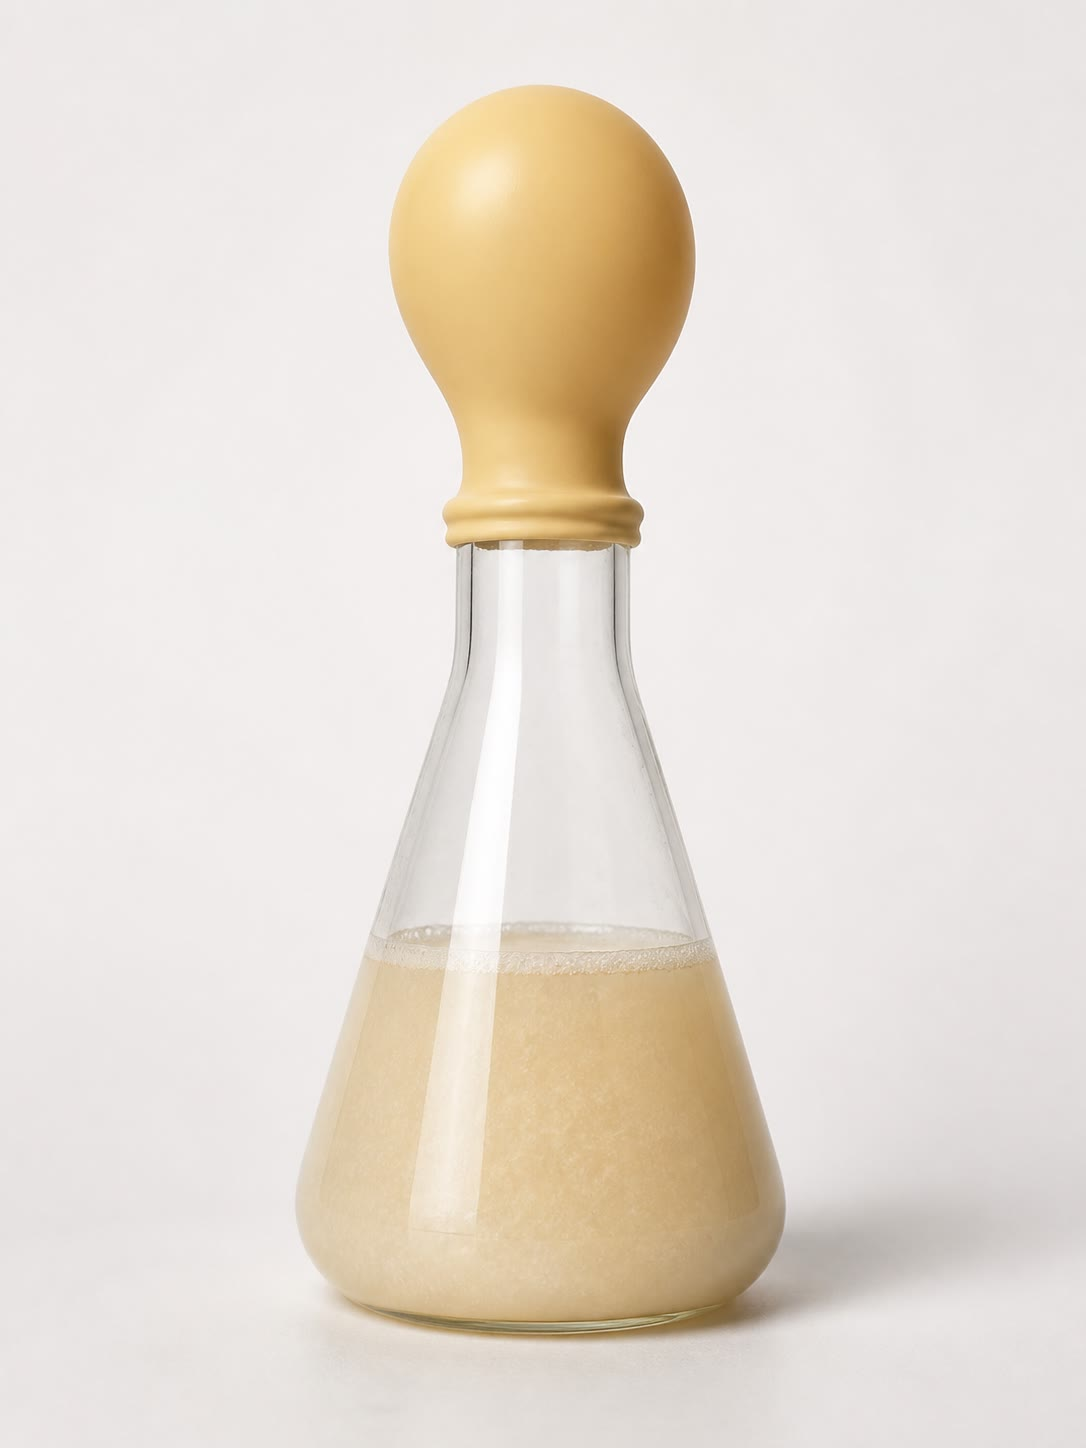
\includegraphics[width=0.36\linewidth]{images/book2/ai/g10-metab-yeast-balloon.jpg}

{\small 烧瓶中酵母\omterm{def:g10:cell-metabolism:fermentation}{发酵}\omterm{def:g10:chemistry-of-life:families}{糖类}：酒精\omterm{def:g10:cell-metabolism:fermentation}{发酵}产生的二氧化碳
使气球膨胀。液体中无氧，
糖只被部分分解，乙醇
则留在其中。}
\end{omfigure}

\begin{example}[空气中与无空气时的酵母]\label{ex:g10:cell-metabolism:pasteur}
通入空气的酵母节省地利用葡萄糖，生长迅速：它
进行呼吸作用。同样的酵母置于密闭大桶中，大量消耗葡萄糖，生长
很慢，并产生乙醇：它进行\omterm{def:g10:cell-metabolism:fermentation}{发酵}。巴斯德于
1861 年描述此现象，称\omterm{def:g10:cell-metabolism:fermentation}{发酵}为“无空气的生命”；
\omterm{def:g10:cells-common-unit:cell}{细胞}会将\omterm{def:g10:cell-metabolism:metabolism}{代谢}切换到环境允许的任一途径，由于
\omterm{def:g10:cell-metabolism:fermentation}{发酵}每分子葡萄糖提供的能量极少，它们必须
消耗多得多的糖才能生存。
\end{example}

\begin{omfigure}
\begin{tikzpicture}[>=Stealth, font=\small,
  cell/.style={draw, rounded corners, thick, minimum height=1.5cm, text width=2.7cm, align=center},
  inp/.style={text width=2.3cm, align=right, anchor=east},
  outp/.style={text width=2.6cm, align=left, anchor=west}]
  \node[cell, fill=omMeth!12] (a) at (0,0) {\textbf{自养细胞}\\ 叶绿体};
  \node[inp] (ai) at (-2.2,0) {$\mathrm{CO_2}$、$\mathrm{H_2O}$，\\ 无机盐，\\ \emph{光}};
  \node[outp] (ao) at (2.2,0) {有机物 \\ （葡萄糖、淀粉\dots）\\ $+ \mathrm{O_2}$};
  \draw[->] (ai) -- (a); \draw[->] (a) -- (ao);
  \node[cell, fill=omThm!10] (h) at (0,-3.2) {\textbf{任一细胞}\\ 线粒体};
  \node[inp] (hi) at (-2.2,-3.2) {有机物 \\ $+ \mathrm{O_2}$};
  \node[outp] (ho) at (2.2,-3.2) {$\mathrm{CO_2}$、$\mathrm{H_2O}$\\ $+$ 能量（ATP、热量）};
  \draw[->] (hi) -- (h); \draw[->] (h) -- (ho);
  \node[anchor=west, font=\small\itshape] at (8.6,0) {光合作用};
  \node[anchor=west, font=\small\itshape] at (8.6,-3.2) {呼吸作用};
  \draw[->, gray, thick] (4.6,-0.7) to[bend left=35] node[right, font=\scriptsize, text width=3.6cm, align=left, xshift=2pt] {有机物供给异养生物，以及自养生物自身的呼吸作用} (4.6,-2.5);
\end{tikzpicture}

{\small \omterm{def:g10:cells-common-unit:cell}{细胞}\omterm{def:g10:cell-metabolism:metabolism}{代谢}的两个过程。\omterm{def:g10:cell-metabolism:autotrophy}{光合作用}将光
能储存在\omterm{def:g10:chemistry-of-life:mineral-organic}{有机物}中；呼吸作用则在每个\omterm{def:g10:cells-common-unit:cell}{细胞}中释放能量。
\omterm{def:g10:cell-metabolism:autotrophy}{自养}生物两者兼有；\omterm{def:g10:cell-metabolism:autotrophy}{异养}生物只进行后者，且必须摄入
\omterm{def:g10:chemistry-of-life:mineral-organic}{有机物}。}
\end{omfigure}

\section{决定细胞代谢的因素}

\begin{proposition}[基因与环境]\label{prop:g10:cell-metabolism:decides}
\omterm{def:g10:cells-common-unit:cell}{细胞}的\omterm{def:g10:cell-metabolism:metabolism}{代谢}取决于两个方面：一是其
\emph{装备}——\omterm{def:g10:universal-dna:gene}{基因}允许其构建的酶和\omterm{def:g10:cells-common-unit:organelle}{细胞器}，
以致无叶绿素的\omterm{def:g10:cells-common-unit:cell}{细胞}永远不能进行\omterm{def:g10:cell-metabolism:autotrophy}{光合作用}
——二是其\emph{环境}——光照、氧气、可用的
营养物质——它决定可能的\omterm{def:g10:cell-metabolism:metabolism}{代谢}途径中哪些真正
进行。酵母在有空气时进行呼吸，无空气时进行\omterm{def:g10:cell-metabolism:fermentation}{发酵}；
\emph{Euglena} 在光下为\omterm{def:g10:cell-metabolism:autotrophy}{自养}生物，在
黑暗中为\omterm{def:g10:cell-metabolism:autotrophy}{异养}生物；绿色植物的根\omterm{def:g10:cells-common-unit:cell}{细胞}终生为\omterm{def:g10:cell-metabolism:autotrophy}{异养}，由
叶片供给。
\end{proposition}
\admitted

\begin{method}[读取代谢曲线]\label{met:g10:cell-metabolism:trace}
氧探针实验给出浓度随时间的变化。
\begin{enumerate}
  \item 找出每个标记时刻发生了什么变化（开灯、
        加入底物、氧气耗尽）。
  \item 读取每段直线的斜率：升高量与时间之比，以
        \unit{mg/L} 每分钟计。斜率为正表示氧气净产生，
        斜率为负则表示氧气净消耗。
  \item 注意，进行\omterm{def:g10:cell-metabolism:autotrophy}{光合作用}的\omterm{def:g10:cells-common-unit:cell}{细胞}同时进行呼吸：光照下的斜率
        等于产生量减去呼吸消耗，因此\omterm{def:g10:cell-metabolism:autotrophy}{光合作用}的真实速率
        为光照下斜率加上黑暗中的
        斜率的绝对值。
  \item 如需换算：在这些浓度下，\qty{1}{mg/L} 溶解氧
        相当于 $1/32$ 毫摩尔每升。
\end{enumerate}
\end{method}

\begin{example}[藻类的真实速率]\label{ex:g10:cell-metabolism:truerate}
在 \emph{Chlorella} 图中，光照下氧气增加了 \qty{2.5}{mg/L}，
共 5 分钟（斜率 $+0.5$）；黑暗中减少了 \qty{0.5}{mg/L}，共
5 分钟（斜率 $-0.1$）。光照下呼吸作用同样消耗 \qty{0.1}{mg/L}
每分钟，因此\omterm{def:g10:cell-metabolism:autotrophy}{光合作用}产生
$0.5 + 0.1 = \qty{0.6}{mg/L}$ 每分钟，是呼吸消耗量的
六倍。藻类为氧气与\omterm{def:g10:chemistry-of-life:mineral-organic}{有机物}的净生产者，这也是它能生长的
原因。
\end{example}

\section{练习}

\begin{exercise}[$\star$]\label{exo:g10:cell-metabolism:1}
给出\omterm{def:g10:cell-metabolism:metabolism}{代谢}的定义，并说明什么是酶以及酶的作用。
\end{exercise}

\begin{exercise}[$\star$]\label{exo:g10:cell-metabolism:2}
写出\omterm{prop:g10:cell-metabolism:respiration}{细胞呼吸}和\omterm{def:g10:cell-metabolism:autotrophy}{光合作用}的总反应式，
并说明二者在哪些意义上互为逆过程，
在哪些方面又并非如此？
\end{exercise}

\begin{exercise}[$\star$]\label{exo:g10:cell-metabolism:3}
判断下列生物或\omterm{def:g10:cells-common-unit:cell}{细胞}属于\omterm{def:g10:cell-metabolism:autotrophy}{自养}还是\omterm{def:g10:cell-metabolism:autotrophy}{异养}：蘑菇、苔藓、胡萝卜的根\omterm{def:g10:cells-common-unit:cell}{细胞}，
chlorella、酸奶中的细菌、人体肌肉\omterm{def:g10:cells-common-unit:cell}{细胞}。
\end{exercise}

\begin{exercise}[$\star$]\label{exo:g10:cell-metabolism:4}
在酵母与气球的实验中，什么气体使气球膨胀，
什么液体产物会积累，以及烧瓶缺少什么
会改变实验结果？
\end{exercise}

\begin{exercise}[$\star$]\label{exo:g10:cell-metabolism:5}
为什么煮沸过的肝脏不再使过氧化氢冒泡？
\end{exercise}

\begin{exercise}[$\star\star$]\label{exo:g10:cell-metabolism:6}
在酵母图中，氧气在第 3 至第 10 分钟之间，由 \qty{7.9}{mg/L} 降至
\qty{0.9}{mg/L}。计算
以 \unit{mg/L} 每分钟表示的呼吸速率。为何
曲线在第 10 分钟后趋于平缓？此时酵母在做什么？
\end{exercise}

\begin{exercise}[$\star\star$]\label{exo:g10:cell-metabolism:7}
Chlorella 在光照下氧气斜率为 $+0.8$ \unit{mg/L}
每分钟，黑暗中为 $-0.2$。计算\omterm{def:g10:cell-metabolism:autotrophy}{光合作用}速率。
\end{exercise}

\begin{exercise}[$\star\star$]\label{exo:g10:cell-metabolism:8}
一个\omterm{prop:g10:cell-metabolism:respiration}{细胞呼吸}消耗了 \qty{18}{g} 葡萄糖。它消耗多少质量的氧气，
并释放多少质量的二氧化碳？（摩尔质量：
葡萄糖 \qty{180}{g/mol}，$\mathrm{O_2}$ \qty{32}{g/mol}，
$\mathrm{CO_2}$ \qty{44}{g/mol}。）
\end{exercise}

\begin{exercise}[$\star\star$]\label{exo:g10:cell-metabolism:9}
萌发的豌豆置于保温瓶中，一天内使瓶温升高
\qty{4}{\celsius}；煮沸过的豌豆则不会。解释两种结果，
并说明为什么保温瓶不能密闭。
\end{exercise}

\begin{exercise}[$\star\star$]\label{exo:g10:cell-metabolism:10}
将一片绿叶在黑暗中放置 48 小时，然后将其一半
用黑纸遮盖，植株再置于阳光下一天。
滴加碘液。预测并解释两半叶片的结果，
并说明为何需要 48 小时的黑暗处理。
\end{exercise}

\begin{exercise}[$\star\star$]\label{exo:g10:cell-metabolism:11}
解释为什么密闭\omterm{def:g10:cell-metabolism:fermentation}{发酵}罐中的酵母，按每个\omterm{def:g10:cells-common-unit:cell}{细胞}计，
消耗糖的速度远快于通入空气的酵母。
\end{exercise}

\begin{exercise}[$\star\star\star$]\label{exo:g10:cell-metabolism:12}
短跑运动员参加 400 米比赛后，肌肉会变得酸痛并呈酸性。
解释肌肉\omterm{def:g10:cells-common-unit:cell}{细胞}中发生了什么、发生的原因，
以及同一运动员慢跑时肌肉为何不会变酸。
\end{exercise}

\begin{exercise}[$\star\star\star$]\label{exo:g10:cell-metabolism:13}
\emph{Euglena} 在有机食物的黑暗环境中放置一个月后失去了\omterm{def:g10:cells-common-unit:organelle}{叶绿体}，
但其后代在光照下又重新获得了\omterm{def:g10:cells-common-unit:organelle}{叶绿体}。在
\cref{prop:g10:cell-metabolism:decides}中的两个因素里，哪一个发生了变化，
哪一个没有？这次恢复能证明\omterm{def:g10:cells-common-unit:cell}{细胞}的
\omterm{def:g10:universal-dna:gene}{基因}的什么？
\end{exercise}

\begin{exercise}[$\star\star\star$]\label{exo:g10:cell-metabolism:14}
一个密封的鱼缸内装有水、一只蜗牛和一株水生植物，置于光照下。
解释这两种生物各自如何能存活数月，
各自为对方提供了什么，
以及若将鱼缸放在黑暗中会发生什么。
\end{exercise}

\begin{exercise}[$\star\star\star$]\label{exo:g10:cell-metabolism:15}
一分子葡萄糖经呼吸作用约产生 30 个 ATP，\omterm{def:g10:cell-metabolism:fermentation}{发酵}则产生 2 个。一个
酵母\omterm{def:g10:cells-common-unit:cell}{细胞}每分钟需要固定数量的 ATP 才能维持生命。
计算其\omterm{def:g10:cell-metabolism:fermentation}{发酵}时每分钟需多消耗多少倍的葡萄糖；
再解释为何酿酒者要让\omterm{def:g10:cell-metabolism:fermentation}{发酵}罐隔绝空气，
即使这会“浪费”糖。
\end{exercise}

\section{问题：酿酒师的发酵罐}

\begin{problem}[{周末问题——一罐交由酵母发酵的葡萄汁：
其中所含的酒精、放出的气体、产生的热量，
以及酒窖为何可能是危险场所}]
\label{pb:g10:cell-metabolism:1}
葡萄醪每升约含糖 \qty{200}{g}，
视作葡萄糖，\omterm{def:g10:cell-metabolism:fermentation}{发酵}罐一经密封便不含溶解氧。
摩尔质量：葡萄糖 \qty{180}{g/mol}，乙醇
$\mathrm{C_2H_5OH}$ \qty{46}{g/mol}，二氧化碳 \qty{44}{g/mol}，
氧气 \qty{32}{g/mol}。乙醇的密度为 \qty{0.79}{g/mL}。
酒窖温度下，一摩尔气体约占 \qty{24}{L}。
\omterm{def:g10:cell-metabolism:fermentation}{发酵}罐的容积为 \qty{1000}{L}。

\medskip
\noindent\textbf{第一部分——酵母产生了什么。}
\begin{enumerate}
  \item 酵母在密封\omterm{def:g10:cell-metabolism:fermentation}{发酵}罐中采用哪条\omterm{def:g10:cell-metabolism:metabolism}{代谢}途径？为何如此？
        写出其反应式。
  \item 每升葡萄醪含有多少摩尔葡萄糖？
  \item 计算每升产生的乙醇质量，再求其
        体积，然后求葡萄酒的酒精含量，以体积
        百分数计。
  \item 计算每升葡萄醪产生的二氧化碳质量，
        以及其作为气体时的体积。
  \item 对整个\omterm{def:g10:cell-metabolism:fermentation}{发酵}罐，释放的二氧化碳体积为多少？
        与一座 \qty{4}{m} × \qty{6}{m}
        × \qty{2.5}{m} 的酒窖容积相比。
\end{enumerate}

\medskip
\noindent\textbf{第二部分——若酵母能获得空气。}
\begin{enumerate}[resume]
  \item 若葡萄醪持续通气，写出酵母所遵循的
        反应式。
  \item 计算呼吸分解一升葡萄醪中的糖所需氧气的质量，
        以及释放的二氧化碳质量。
  \item 比较第 7 题中的二氧化碳与
        第 4 题中的二氧化碳，并从葡萄糖被分解的
        彻底程度解释其差异。
  \item 呼吸作用每分子葡萄糖约产生 30 个 ATP，\omterm{def:g10:cell-metabolism:fermentation}{发酵}约产生
        2 个。若酵母两种情况下需要相同的 ATP，则哪种情况
        下糖的持续时间更长？相差多少倍？
  \item 解释为何酿酒者仍要隔绝空气。
\end{enumerate}

\medskip
\noindent\textbf{第三部分——\omterm{def:g10:cell-metabolism:fermentation}{发酵}罐的热量。}
\omterm{def:g10:cell-metabolism:fermentation}{发酵}每摩尔葡萄糖约释放 \qty{70}{kJ} 热量；
使 \qty{1}{kg} 水升温 \qty{1}{\celsius} 需要 \qty{4.2}{kJ}。
\begin{enumerate}[resume]
  \item 计算每升葡萄醪释放的热量，再求
        整个\omterm{def:g10:cell-metabolism:fermentation}{发酵}罐释放的热量。
  \item 若热量全部未散失，\omterm{def:g10:cell-metabolism:fermentation}{发酵}罐温度会升高多少？
        （将葡萄醪视为水。）
  \item 酵母的酶在高于约 \qty{40}{\celsius} 时会被破坏。
        从 \qty{20}{\celsius} 开始，未经冷却的\omterm{def:g10:cell-metabolism:fermentation}{发酵}罐能否存活？
        这说明了大型\omterm{def:g10:cell-metabolism:fermentation}{发酵}罐为何
        需要降温？
  \item 利用\cref{prop:g10:cell-metabolism:enzymes}，解释为何
        热量会使\omterm{def:g10:cell-metabolism:fermentation}{发酵}停止，尽管糖仍然存在。
  \item 若进行呼吸作用，每摩尔葡萄糖约会释放 \qty{2870}{kJ}。
        \omterm{def:g10:cell-metabolism:fermentation}{发酵}\emph{没有}释放的那部分能量
        仍留在何处？
\end{enumerate}

\medskip
\noindent\textbf{第四部分——酒窖。}
\begin{enumerate}[resume]
  \item 二氧化碳的密度大于空气。它会在酒窖的哪个位置积聚？
        为何把点燃的蜡烛放低，可作为一种传统的
        安全检测？
  \item 工人的\omterm{def:g10:cells-common-unit:cell}{细胞}缺氧时，会转而采用哪条途径——
        为何人体不能依靠它维持
        超过几分钟？
  \item 当酒精达到体积分数约 15\% 时，\omterm{def:g10:cell-metabolism:fermentation}{发酵}会自行停止。
        试从酵母的酶的角度
        提出一种解释。
  \item 面包面团使用同样的酵母\omterm{def:g10:cell-metabolism:fermentation}{发酵}一小时。面包
        瓤中的气泡含有什么？乙醇在烘烤后
        去了哪里？
  \item 请给出结论：对于一升葡萄醪，其酒精含量
        与所产气体的体积——以及同时解释二者的
        唯一\omterm{def:g10:cell-metabolism:metabolism}{代谢}事实。
\end{enumerate}
\end{problem}
